% !TEX root = ../Vorlage_DA.tex
%	########################################################
% 							Arbeitstitel
%	########################################################


%	--------------------------------------------------------
% 	Überschrift, Inhaltsverzeichnis
%	--------------------------------------------------------
\chapter*{Thema: \newline \htlArbeitsthema }



%	--------------------------------------------------------
% 	Bearbeiter
%	--------------------------------------------------------
\section*{Subtopics and Editor:}


\textbf{Implementing SLAMS and DeepTAM, Image Pre-Processing}\\ 
Alexander Voglsperger, 5AHELS\\
\emph{Advisors:} Dipl. Ing. Müller Gerhard\\[2ex] 
%
\textbf{Implementing DeepTAM, Gathering Trainingdata}\\ 
Simon Moharitsch, 5AHELS\\
\emph{Advisors:} Dipl. Ing. Müller Gerhard\\[2ex]



%	--------------------------------------------------------
% 	Beteiligte Firmen
%	--------------------------------------------------------
\section*{Projectpartner:}

\renewcommand{\arraystretch}{1.5}
\begin{tabularx}{1\textwidth}{@{} l X @{}}

\emph{Designation:} & Johannes Kepler University - Artificial Intelligence Lab\\
\emph{Address:} & Altenberger Straße 69\\
\emph{ZIP, location:} & 4040 Linz, Austria\\
\emph{Contact person:} & Dr. Nessler Bernhard\\
\emph{Phone:} & +43 (0)732 2468 4539\\
\emph{E-Mail:} & nessler@ml.jku.at\\

\end{tabularx}


%--------------------------------------------------------------------------------
%  Vorgeschriebene Dokumentationsseiten
%--------------------------------------------------------------------------------

\pagebreak
\thispagestyle{empty}
\newgeometry{top=2cm, bottom=1.5cm}

\begin{minipage}[c]{0.20\linewidth}

\includegraphics[width=0.8\linewidth]{media/images/htl_c_cmyk_rein}
\end{minipage}
\begin{minipage}[c]{0.6\linewidth}
\begin{center}
{\bfseries\sffamily\large Höhere  technische  Bundeslehranstalt\\
und  Bundesfachschule  Braunau\\
Elektronik und Technische Informatik\\
{\normalsize School autonomous focus on Mobile Computing and Software Engineering} }
\end{center}
\end{minipage}
\begin{minipage}[c]{0.2\linewidth}
\hfill 
\includegraphics[width=0.8\linewidth]{media/images/htl-bildung-mit-zukunft}
\end{minipage}\\

\vspace{1em}
\begin{center}
\bfseries\sffamily\Large
DIPLOMA DOCUMENTATION
\end{center}
\vspace{1ex}

\renewcommand{\arraystretch}{2}
\begin{tabularx}{1\textwidth}{ p{3.5cm} X }

\textbf{Author} & 
Alexander Voglsperger, Simon Moharitsch \\

\textbf{Vintage\linebreak School year} & 
5AHELS 2019/2020 \\

\textbf{\mbox{Topic of the } \mbox{diploma documentation}} & 
\htlArbeitsthema \\

\textbf{Cooperation\-partner} &
Johannes Kepler University - Artificial Intelligence Lab\\

\textbf{Task definition} & 
{The task of this work is to get depth information out of a video stream in real time. The considered field of application is an autonomous driving car that uses several cameras to orientate itself while driving.}\\

\textbf{Realization} & 
{Simultaneous Localization And Mapping (\gls{slam}) algorithms are implemented on the free available platform Robot Operating System (\gls{ros}). ORB-\gls{slam} and LSD-\gls{slam} are two specific SLAM methods. These two slams have been modified to get executable program code on \gls{ros}. Several performance tests and a comparison between ORB-\gls{slam} and LSD-\gls{slam} are also part of this work.} \\

\textbf{Outcome} & 
{In this thesis the result of ORB-\gls{slam} and the LSD-\gls{slam} are compared. The ORB-\gls{slam} is working, but will not produce a detailed map if prominent points are missing in the video. Prominent points are points, edges that stand out of its surroundings and such are a way the \gls{slam}s can get information. The LSD-\gls{slam} does not work as good as the ORB-\gls{slam} when the camera only has a axial movement in the sense that it will not react on movement and thus generates an incorrect map. As a result the LSD-\gls{slam} only works on cars when a wide-angle camera lens is used. The problem with DeepTAM it has not been updated recently and because of that there are many compatibility issues with newer drivers, newer Tensor Flow framework and other required libraries.} \\

\end{tabularx}

%--------------------------------------------------------------------------------

\pagebreak
\thispagestyle{empty}
\newgeometry{top=2cm, bottom=1.5cm}


\begin{minipage}[c]{0.20\linewidth}

\includegraphics[width=0.8\linewidth]{media/images/htl_c_cmyk_rein}
\end{minipage}
\begin{minipage}[c]{0.6\linewidth}
\begin{center}
{\bfseries\sffamily\large Höhere  technische  Bundeslehranstalt\\
und  Bundesfachschule  Braunau\\
Elektronik und Technische Informatik\\
{\normalsize School autonomous focus on Mobile Computing and Software Engineering} }
\end{center}
\end{minipage}
\begin{minipage}[c]{0.2\linewidth}
\hfill 
\includegraphics[width=0.8\linewidth]{media/images/htl-bildung-mit-zukunft}
\end{minipage}\\

\vspace{1em}

\renewcommand{\arraystretch}{2}
\begin{tabularx}{1\textwidth}{ p{3.5cm} X }

\textbf{\mbox{Illustrative graph,} \mbox{photo} \mbox{(incl. explanation)}} & 
{
Structure of the flowchart:
\begin{center}
	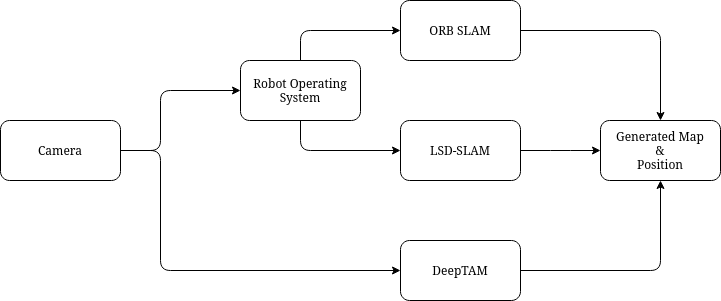
\includegraphics[width=1\linewidth]{media/images/illustrative_graph.png}
\end{center}
} \\
  
%\textbf{\mbox{Participation in} competitions, Awards} & 
%{
%Participated:
%\begin{itemize}
%\item Jugend Innovativ
%\item ITs Award
%\item FH Kärnten Maturaprojekt-Wettbewerb
%\item computer creative wettbewerb
%\item 120 Sekunden Wettbewerb
%\end{itemize}
%} \\

\textbf{\mbox{Accessibility of} \mbox{diploma thesis}} & 
{HTL Braunau archive, or\newline \url{https://diplomarbeiten.berufsbildendeschulen.at/}} \\



\end{tabularx}




%--------------------------------------------------------------------------------
% Unterschriften
%--------------------------------------------------------------------------------



\vspace*{\fill}

\textbf{Approval (date / signature)}

\fbox{
\begin{minipage}[t][3cm]{0.5\linewidth}
\centering
    Examiner \\
    %\hspace*{\fill}\includegraphics[width=0.8\linewidth]{fig/Unterschrift}\hspace*{\fill}
    \vfill
    \end{minipage}}
    \fbox{
    \begin{minipage}[t][3cm]{0.5\linewidth}
    \centering
    Head of College / Department
    \vfill
\end{minipage}
}

\restoregeometry

